\chapter{Hardware}\label{ch:foundation}
\epigraph{Day by day, what you choose, what you think and what you do is who you become.}{--- Heraclitus}
\section{Game environment}\label{sec:game_environment}
As mentioned in section~\ref{sec:research_question}, we were interested in understanding phenomena related to player engagement in~\gls{pirg}s with a mobile adversarial robot. For that, we had chosen to use RoboTower~\citep{bonarini_timing_2014} as a starting point, perfecting the interaction and playability.

A main difference concerns the playground, which in our case consisted of a rectangular area of 4m$\times$4m, and the extinction of cards as mean of interaction. Here, we used the player's proximity instead as interaction channel. On each corner of the playground, tubes (henceforth called ``towers'') were placed. Each tower was equipped with a button (which sits on the tower's cap) and four~\gls{led}s that could be progressively turned on, one by one.  Each~\gls{led} required the button to be pressed for 2.5 seconds, meaning that the tower took about 10 seconds of button push in order to light up all of its four~\gls{led}s.

The~\gls{led}s are supposed to display the progress of the human player in capturing a specific tower. For a given tower, after turning on all~\gls{led}s, it is said that the player had captured it; Figure~\ref{tubes} presents the towers that were used in the game. When a tower is secured, the robot cannot aim at it anymore.
Button pressing time was cumulative and could be distributed on different moments -- that meant that the player would not lose his progress if he stopped pressing the button before the tower is completely captured. 

The game mechanics and winning conditions were simple enough to allow for a large number of individual playing the game. In order to win, the human players must be able to secure all the existing towers without letting a single one be knocked down by the robot. If, at anytime, a tower falls (because of the robot or the player) the game ends and the human player loses. 

The robot was able to move across the entire playground just as the human player could and it was only constrained by the fact that an already captured tower, or one whose button is currently being pressed by the player, cannot be teared down. As main interaction channel between the two players,\ie robot and human, the human player could block the robot path at any moment by staying in front of it, causing the later to likely change target tower. Therefore, as consequence of the defined rules, while the player was trying to capture a given tower, the robot could try to tear down any other one.

%ANDY This would go in the robot description -> By relying on the lasers scans the robot can perceive its environment, locate itself and the human player during the game, being able to perform obstacle avoidance when appropriated.

The game definition in itself is no trivial task and it is, for the case of~\gls{pirg}, limited by the constraints imposed by the mechanical platform,~\ie the robot. Other than playability and fun, safety is also an important aspect and one that impose heavy bounds to the motion of the robot: a too fast of a robot would reduce the perception of the robot been safe too play against, thus limit the interaction. Experimentally, we have evaluated that a robot with a maximum linear speed of 1.4 m/sec would be too difficulty to play against and/or invincible (which is not the behavior we were looking for). Intuitively, as we allowed an increase in speed, an impact in difficulty would be perceive. Moreover, for a mobile robot as ours, speed have some negative impact in the robot control itself, through mechanical phenomena like wheel slippage, initial control, manoeuvrability, and navigation issues (localization and obstacle avoidance). Details about the robot platform is given in section~\ref{sec:roboplat}.

In summary, our game, called RoboTower v2, was designed such that we could have an environment rich enough to physically engage human players while allowing for the study of adaptive approaches towards supporting such engagement. RoboTower v2 stimulates player to maintain strong cognitive tasks, like: trajectory planning, attention and spatial reasoning and places itself as an interesting environment from which one could test~\gls{ml} approaches. Next we briefly detail the Towers used in the game in term of their properties and operating system.
%ANDY Here is one of the places were the smartness of game design has to be put in evidence.

%\begin{figure}[H]
%	\centering
%	\begin{subfigure}[b]{0.4\textwidth}
%		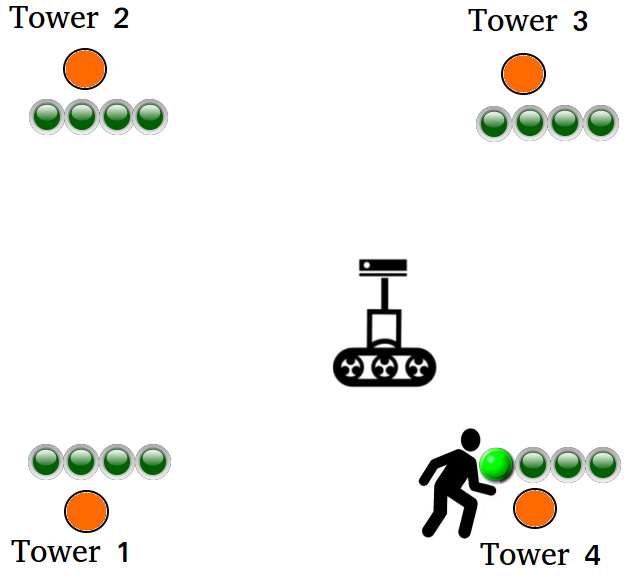
\includegraphics[width=5cm]{Chapter4/Figs/situation1}
%		\caption{Initial situation: player is capturing Tower-4}
%		\label{situation1} 
%	\end{subfigure}
%	\begin{subfigure}[b]{0.4\textwidth}
%		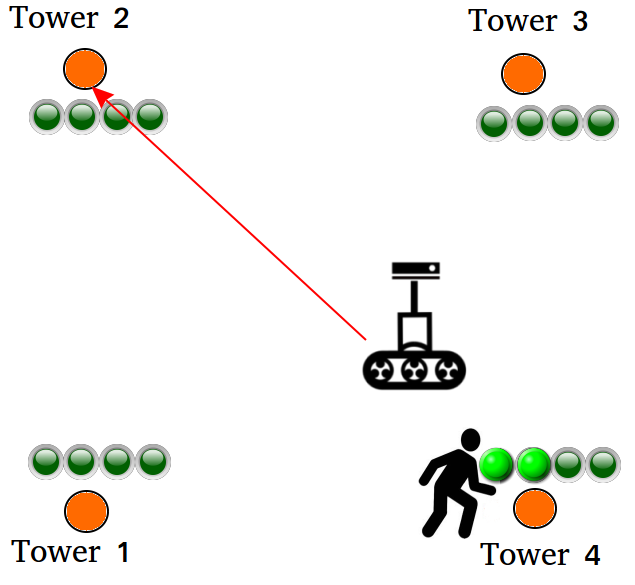
\includegraphics[width=5cm]{Chapter4/Figs/situation2}
%		\caption{Robot start moving in order to attack and tear down Tower-2}
%		\label{situation2}
%	\end{subfigure}
%	\begin{subfigure}[b]{0.4\textwidth}
%		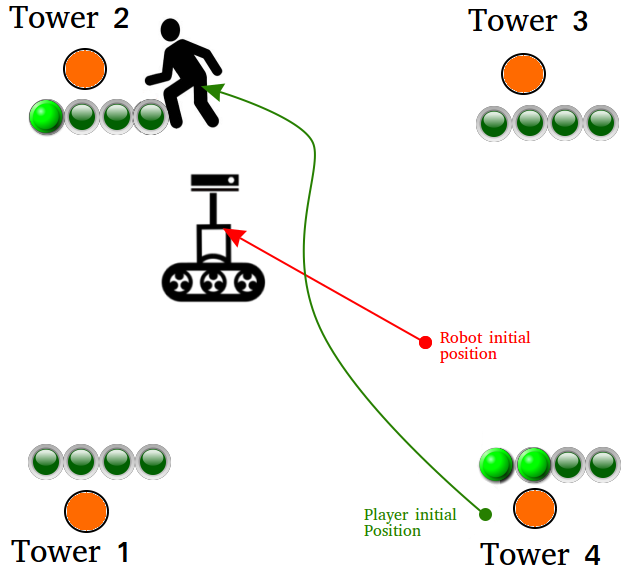
\includegraphics[width=5cm]{Chapter4/Figs/situation3}
%		\caption{Human player defends and start capturing Tower-2} 
%		\label{situation3}
%	\end{subfigure}
%	\begin{subfigure}[b]{0.4\textwidth}\centering
%		\includegraphics[width=3cm]{Chapter4/Figs/tubes}
%		\caption{Real towers that are used during the game}
%		\label{tubes} 
%	\end{subfigure}
%	\rule{35em}{0.5pt}
%	\caption{Schematic representation of the game:}
%	\label{overallgame}
%\end{figure}
%\begin{itemize}
%	\item figure~\ref{situation1}: The player is capturing the tower, when all the four LEDs are lit on the tower.
%	\item figure~\ref{situation2}: The robot attacks a Tower, it cannot try to tear down the tower that is currently being captured by the player.
%	\item figure~\ref{situation3}: The player stops the action of the robot by blocking its trajectory and defending the attacked tower. \textit{Please notice} how the progress on Tower-4 is not lost even if the player dismiss capturing it.
%\end{itemize}

%\begin{figure}[H]
%	\centering
%	\includegraphics[width=10cm]{Chapter5/Figs/im1}
%	\rule{35em}{0.5pt}
%	\caption{Moving robot tracking the movements of a human.}
%	\label{trackingconcept1} 
%\end{figure}

%To obtain the data from the human player that are needed to perform the tracking we used the Microsoft Kinect presented in~\ref{kinectsec} and a computer vision algorithm for blob detection previously integrated in the ROS environment using OpenCV libraries.

\section{Towers}\label{sec:towers}
Each tower was powered individually, being capable of transmitting its status to the robot at a constant rate. The circuit used the~\href{https://einstronic.com/wp-content/uploads/2017/06/NodeMCU-ESP8266-ESP-12E-Catalogue.pdf}{NodeMCU V3 ESP8266 ESP-12E} WiFi module\footnote{\url{https://goo.gl/TzAjwi} accessed on December 17th, 2018.} whose connection was done via a private network. The communication between towers and the robot was supported through TCP protocol using the rosserial\_server\footnote{\url{http://wiki.ros.org/rosserial_server} accessed on December 17th, 2018.} package. Appendix~\ref{app:hard_appendix} provides additional hardware details for the towers. 

As power supply, a $7.4$V LiPo battery was used on each tower as can been seen on figure~\ref{fig:tower_caps}. The nominal voltage for the boards was $5$V, which is supplied through a voltage regulator. A tilt sensor allows for the detection of fallen towers. A schematic of the circuit developed to detect such event is provided in figure~\ref{fig:tilt_circuit}.

\begin{figure}[H]
  \centering
  \begin{subfigure}[t]{0.33\textwidth}
  	\centering
    \includegraphics[width=3cm, height=5cm]{images/03-foundation/cap1}
	\caption{}
  \end{subfigure}
  ~ 
  \begin{subfigure}[t]{0.33\textwidth}
  	\centering
    \includegraphics[width=3cm, height=5cm]{images/03-foundation/cap2}
	\caption{}
  \end{subfigure}
  ~
   \begin{subfigure}[b]{0.33\textwidth}
	  \centering
      \includegraphics[width=3cm,  height=5cm]{images/04-activity/tubes.jpg}
      \caption{}
    \end{subfigure}
  \caption{a) Tower cap containing the button and \gls{led}s; b) Tower cap circuit; c) The four towers used in the game (height 110cm).}
  \label{fig:tower_caps}
\end{figure}


\begin{figure}[H]
	\centering
		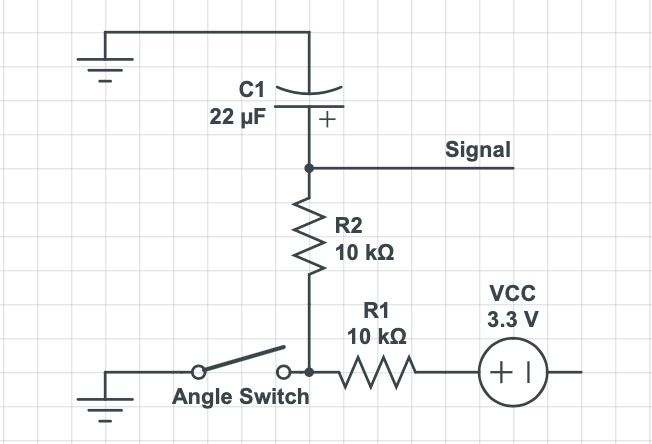
\includegraphics[width=0.4\textwidth, height=5cm]{images/03-foundation/tilt_sensor_circuit}
	\caption{The circuit for detecting when a tower has fallen. An angle switch detects the inclination and the low-pass filter smooths out noise from vibrations such as those caused by the player touching the tower. The signal wire is attached to a pin on the NodeMCU V3 ESP8266 ESP-12E WiFi Module, which allows communication with the robot's onboard computer.}
    \label{fig:tilt_circuit} 
\end{figure}

\section{The robotic platform}\label{sec:roboplat} 
As depicted in figure~\ref{graph:PIRG_design_structure}, hardware is the core concern for a mobile robot in~\gls{pirg}. In the graph in figure~\ref{graph:HARDWARE_structure} we have detailed some concepts of importance considered during our design. The graph is not supposed to give an extensive map of the necessary hardware aspects and their inter relationship, but to instruct the reader on the necessary aspect in this first phase of design taking our development as example. Naturally, not all mobile robots involved in~\gls{pirg}s will take into account all such concerns. In fact, the original RoboTower~\citep{bonarini_timing_2014} and Jedi Trainer 3.0~\citep{martinoia_physically_2013} were examples of mobile robots that did not considered, for instance, navigation techniques, such as~\gls{slam} and~\gls{oa} and had no sophisticated structural and sensing requirements given the little computing power available.

Our wheeled robot, instead, had holonomic kinematics and was called Triskar. Being holonomic, it was free to move in any direction at a speed comparable to that of people in indoor environments (up to 1.4~m/sec). The base consisted of a metallic, triangular-shaped structure where motors, batteries, computer and necessary electronics are embedded. In total, the robot weighed $22.3$ kg. Triskar had simultaneously and independently controlled rotational and translational motion capabilities thanks to three omni-directional wheels actuated by a motor each. The robot's movement on flat floor was as free as the human which made it a good base for adversarial~\gls{pirg}s and, in particular, the one that we had designed. 

\begin{figure}[H]
    \centering
    \begin{tikzpicture}[ every annotation/.style = {draw,
                         fill = white, font = \Large}, scale=0.75,transform shape]
                         
      \path[mindmap,concept color=black!40,text=white,
        every node/.style={concept,circular drop shadow},
        root/.style    = {concept color=black!40,
          font=\large\bfseries,text width=10em},
        level 1 concept/.append style={font=\Large\bfseries,
          sibling angle=90,text width=7.7em,
        level distance=15em,inner sep=0pt},
        level 2 concept/.append style={font=\bfseries,level distance=9em},
      ]
        node[concept, font=\fontsize{20pt}{17pt}\selectfont\bfseries] {Hardware}
        [clockwise from=0]
        child[concept color=blue] {
          node[concept] {Power}
          [clockwise from=-60]
          child { node[concept, font=\fontsize{7pt}{17pt}\selectfont\bfseries] {Consumption} }
          child { node[concept] {Capacity} }
        }
        child[concept color=black] {
            node[concept] {Computing}
            [clockwise from=10]
            child[concept] { node[concept] {Planning} }
            child[concept] { node[concept] {Tracking} }
            child[concept] {
                node[concept,scale=1.5,font=\fontsize{9pt}{17pt}\selectfont\bfseries] {Navigation}
                [clockwise from=250]
                child { node[concept, font=\fontsize{7pt}{17pt}\selectfont\bfseries] {SLAM} }
                child { node[concept, font=\fontsize{8pt}{17pt}\selectfont\bfseries] {OA} }
            }
            child[concept] {
              node[concept] {Sensing}
              [counterclockwise from=150]
              child { node[concept, font=\fontsize{7pt}{17pt}\selectfont\bfseries] {Range} }
              child { node[concept, font=\fontsize{7pt}{17pt}\selectfont\bfseries] {HZ} }
              child { node[concept, font=\fontsize{7pt}{17pt}\selectfont\bfseries] {Cost} }
              child { node[concept, font=\fontsize{7pt}{17pt}\selectfont\bfseries] {Proc} }
            }  
        }
        child[concept color=red] {
            node[concept] {Structure}
            [clockwise from=160, scale=0.8]
            child { node[concept, font=\fontsize{8pt}{17pt}\selectfont\bfseries] {Kinematics}}
            child { node[concept, font=\fontsize{8pt}{17pt}\selectfont\bfseries] {Material}}
            child { node[concept, font=\fontsize{8pt}{17pt}\selectfont\bfseries] {Robustness}}
            child { node[concept, font=\fontsize{8pt}{17pt}\selectfont\bfseries] {Safety}}
        };
    \end{tikzpicture}
    \caption{Some relevant concepts in the hardware dimension for the design of a~\gls{pirg} mobile agent. SLAM stands for Simultaneous localization and Mapping, a set of techniques related to navigation. OA stands for Obstacle Avoidance. Proc and Hz, under sensing, stand for Processing and Frequency respectively.}
    \label{graph:HARDWARE_structure}
\end{figure}

During the research progress, we have designed several versions of our robot, where the first two had an overall height of 85~cm, so comparable to that of a child players, but also acceptable for adult players. The first three versions adopted a Kinect\textsuperscript{\textregistered} sensor on top aimed at player tracking. Given the need to improve robustness, we have redefined the base by making structural changes to limit vibrations and improve stability of the sensors, which increased the overall height to 1 meter (2nd version). We also added new sensors such as planar laser scans needed to obtain reliable obstacle avoidance and localization (3rd and 4th version). Figure~\ref{fig:evolution} depicts our prototype evolution. Finally, on the fourth version we dropped the 3-D camera, deemed to be too much unreliable for player detection, and devised for this goal algorithms based on laser scans only. We kept the height in the same range as before, for the mentioned reasons, although it was no longer needed to hold Kinect\textsuperscript{\textregistered}. To justify the height and give a character to the robot, we added eyes and hair on top, which were appreciated by players. On the next section we expose some consideration regarding sensing.

\begin{figure}[H]
      \centering
      \begin{subfigure}[b]{0.22\textwidth}
      	\centering
	    \framebox{\parbox{2.5cm}{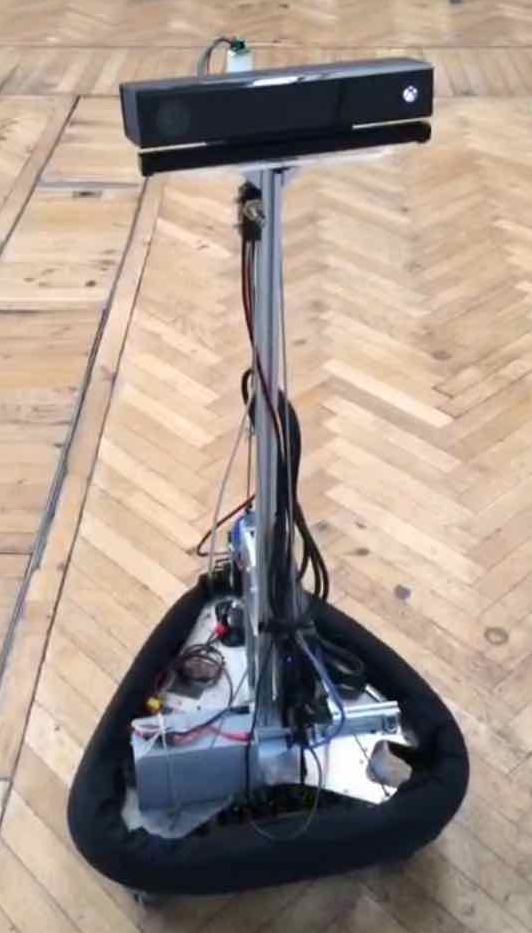
\includegraphics[draft=false,height=4cm,width=2.5cm]{images/03-foundation/triskar1}}}
	  	\caption{}
	  	\label{fig:evolution_a}
      \end{subfigure}
	 ~
	  \begin{subfigure}[b]{0.22\textwidth}
		\centering
	  	\framebox{\parbox{2.5cm}{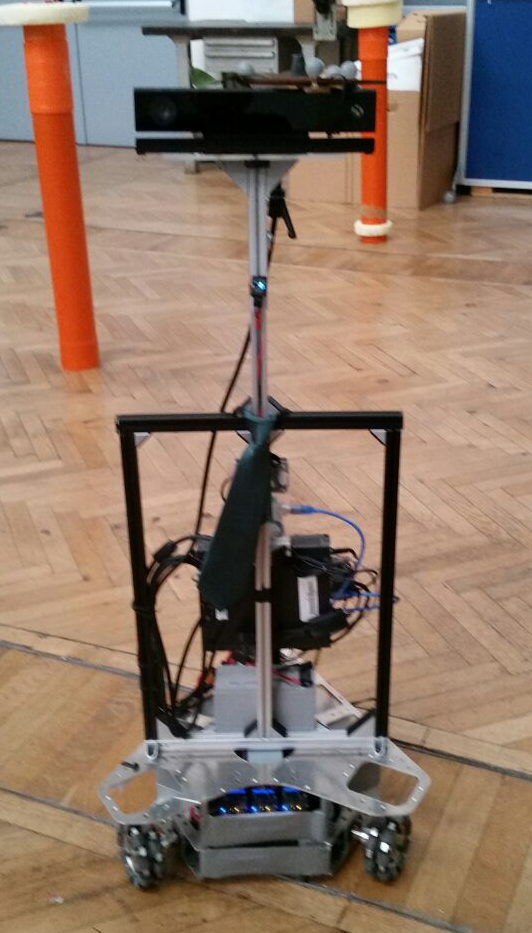
\includegraphics[draft=false,draft=false,height=4cm,width=2.5cm]{images/03-foundation/triskar2}}}
	  	\caption{}\label{robot}
      \end{subfigure}
      ~
      \begin{subfigure}[b]{0.22\textwidth}
      	\centering
      	\framebox{\parbox{2.5cm}{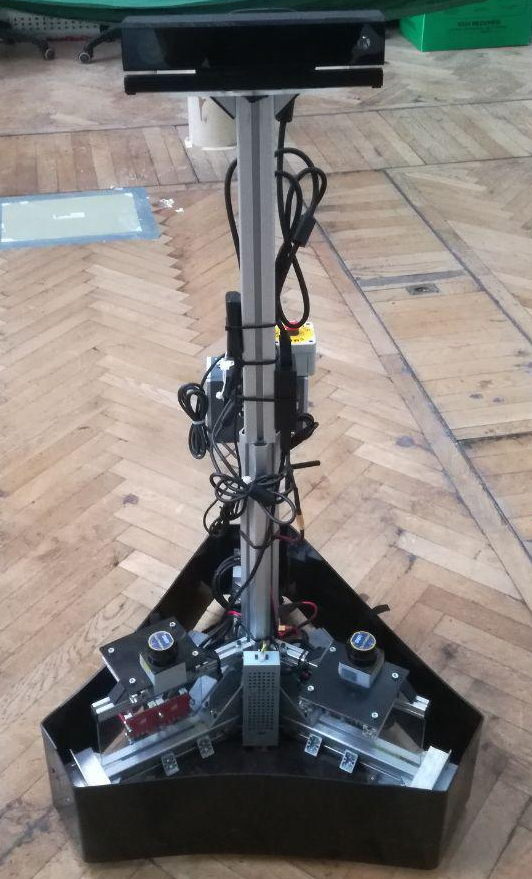
\includegraphics[draft=false,draft=false,height=4cm,width=2.5cm]{images/03-foundation/triskar3}}}\label{newrobot}
      	\caption{}
      \end{subfigure}
      ~
      \begin{subfigure}[b]{0.22\textwidth}
	      \centering
	      \framebox{\parbox{2.5cm}{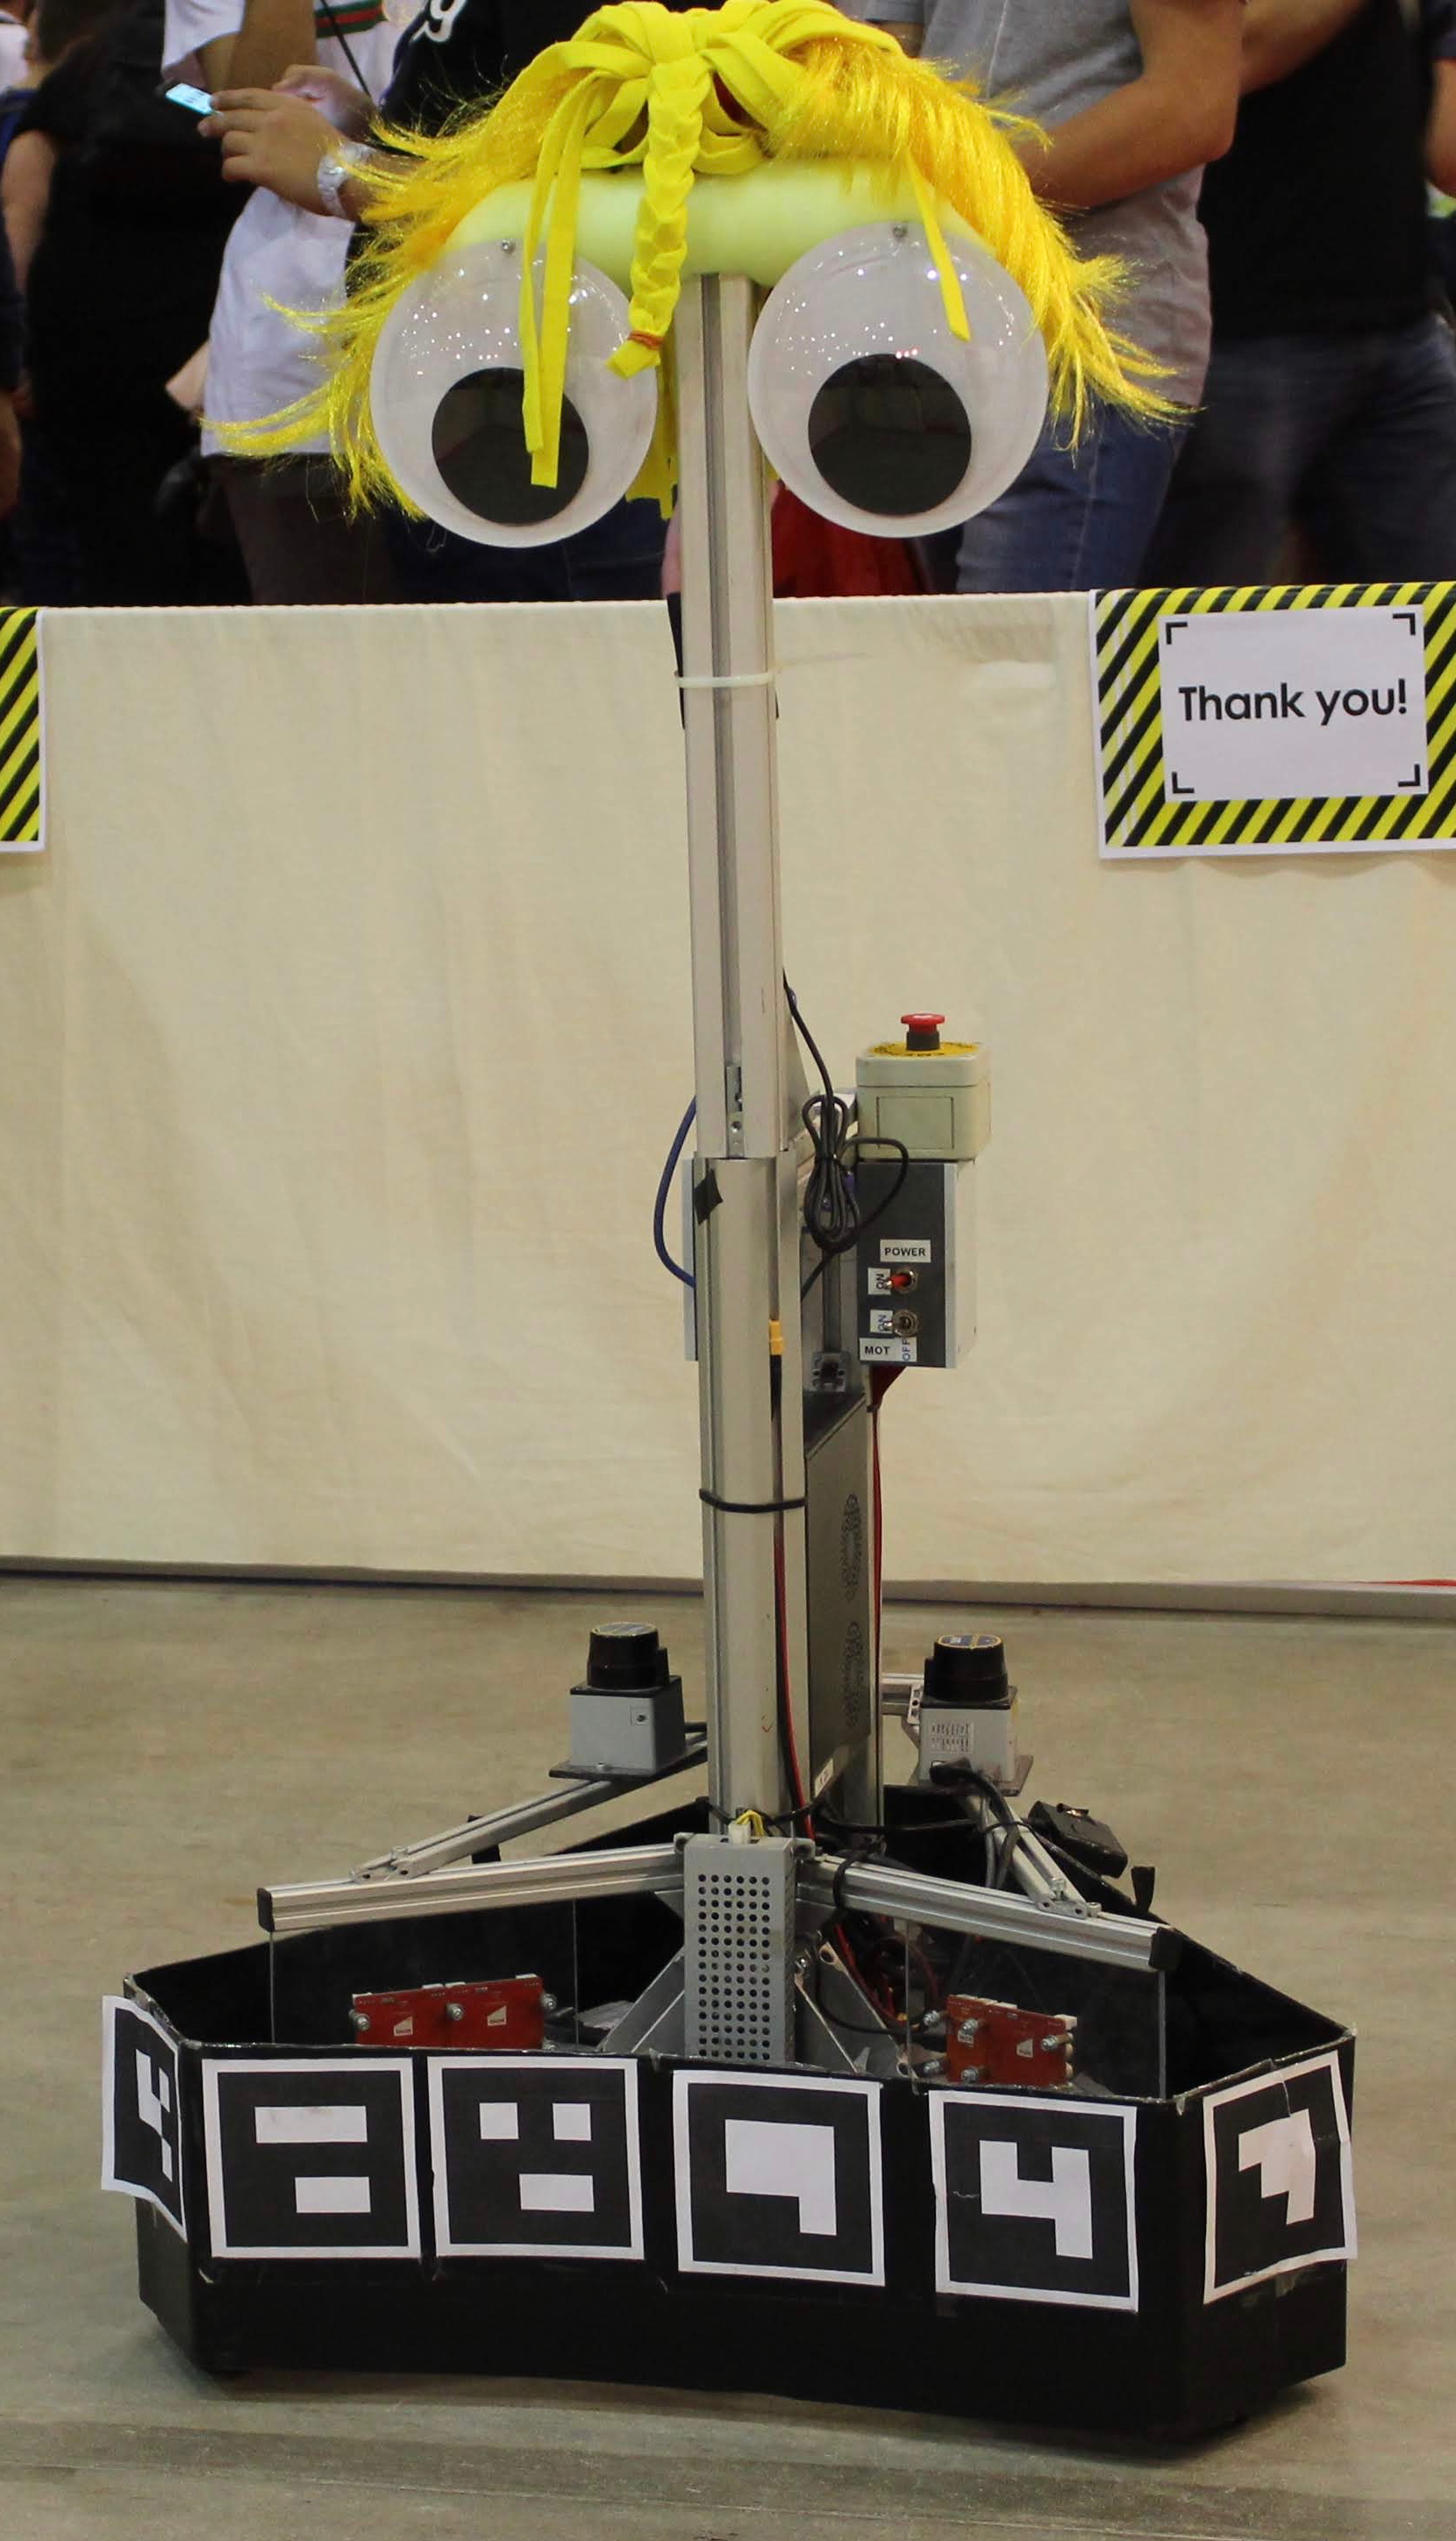
\includegraphics[draft=false,draft=false,height=4cm,width=2.5cm]{images/03-foundation/base4.png}}}\label{newrobot}
	      \caption{}
      \end{subfigure}
      \caption{Prototype evolution. a) First version having the Microsoft Kinect\textsuperscript{\textregistered} camera sensor support secured by steel cables in order to reduce vibration due to motion. b) Second version had improved stability by replacing the steel cables by rigid modular aluminum profiles. c) Third version had a completely redefined base including new electronics, thicker aluminum chassi, redesigned power distribution system and 2D lasers. This version also had a larger base compared to previous prototypes; d) Current version during demonstration at the Maker Faire 2018 in Rome (the European edition) from October 12th to 14th of 2018. A better placement of lasers had made the use of Kinect\textsuperscript{\textregistered} unnecessary since it allowed for full 360\textsuperscript{$\circ$} laser sensing coverage.}
      \label{fig:evolution}
\end{figure}

\subsection{Sensing}
\subsubsection{Microsoft Kinect\textsuperscript{\textregistered}\label{sec:kinectsec}}
In some phases of our development we have used the Microsoft Kinect\textsuperscript{\textregistered} sensor. It is a 3-D camera: in addition to providing an RGB image with its 1080p color camera, it also provides a depth map,  meaning that for every pixel of the depth image provided by the sensor, Kinect\textsuperscript{\textregistered} provides the distance from the sensor (see appendix~\ref{app:hard_appendix} for sensor specifications). This makes the it suitable for a variety of computer vision problems like background removal, blob detection, and people tracking.

\subsubsection{Laser scanners}\label{lasershokuyo}
The robot was equipped with two laser scanners Hokuyo URG-04LX\footnote{\url{https://www.hokuyo-aut.jp/search/single.php?serial=165} accessed on \today}
%, shown in Figure~\ref{fig:hokuyo}
. These laser sensors perceive the range of obstacles on a plan with a field of view of $240^\circ$ and a resolution of $0.36^\circ$, the maximum detectable distance is $5.6m$ and they can be connected to the computer by means of a USB interface, being operated with a nominal voltage of 5V.

The Hokuyo URG-04LX consists of a compact stacked structure with a spindle motor and the actual scanner on top of it. The motor rotates a small transmission mirror that deflects the vertical laser beam coming from the top of the sensor into horizontal direction. This allows the laser beam to scan a planar area around the sensor with an opening angle of $240^\circ$. A second mirror below, the reception mirror, deviates the horizontal laser beam captured by a lens into vertical direction again.

% \begin{figure}[H]
% 	\centering
% 	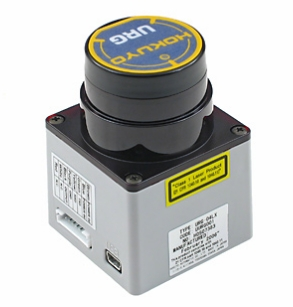
\includegraphics[width=5cm]{images/03-foundation/hokuyo}
% 	\caption{ An Hokuyo URG-04LX laser scanner.}
% 	\label{fig:hokuyo} 
% \end{figure}

A full scan is performed every 100 ms. We mounted a laser scanner on each side of the lower chassis allowing for a $360^\circ$ coverage around the robot at a height of 30 cm from the floor.

\section{Structure \& Materials}
\subsection{Chassis}
The chassis of our robot was made entirely from modular aluminum profiles put together as to define the shape in figure~\ref{fig:aluminum_structure} (3rd prototype). The arrangement of the wheels, as to allow for the holonomic behavior, also allowed us to place batteries conveniently~(see figure~\ref{fig:batteries}) as well as the onboard computer and electronics~(see figure~\ref{fig:computer}). The careful placement of heavyweight elements, such as the lead-acid batteries, turned out to be important in our design since it impacted manoeuvrability. For instance, during test it occurred that, due to inertia, the robot would become vertically unstable when making quick turns or rapidly reacting to the human player's presence. 

The constraint of having the Microsoft Kinect\textsuperscript{\textregistered} sitting on top of a aluminum profile, as to allow maximum visibility from the sensor, moved the center of mass upwards making vertical balance worse. The void created between the wheels, in prototype versions three and four, elegantly provided a way to balance weights and make the robot's center of mass close enough to its base center. Figure~\ref{fig:evolution_a} documents the inefficient weight distribution in the first prototype. In the figure its possible to see the placement of one of the lead-acid batteries in the right side of the base, thus, making the weight distribution asymmetric.

Due to forces acting upon the robot during motion we have used software solutions for velocity smoothing that would increasingly bound speed when accelerating and decelerating. This, together with a proper weight distribution, rendered the robot's motion smooth, improving control, at the benefit of reducing the chances of mechanical breakdown caused by material stress.

\begin{figure}[h]
    \centering
    \begin{subfigure}[b]{0.22\textwidth}
      	\centering
        \framebox{\parbox{2.5cm}{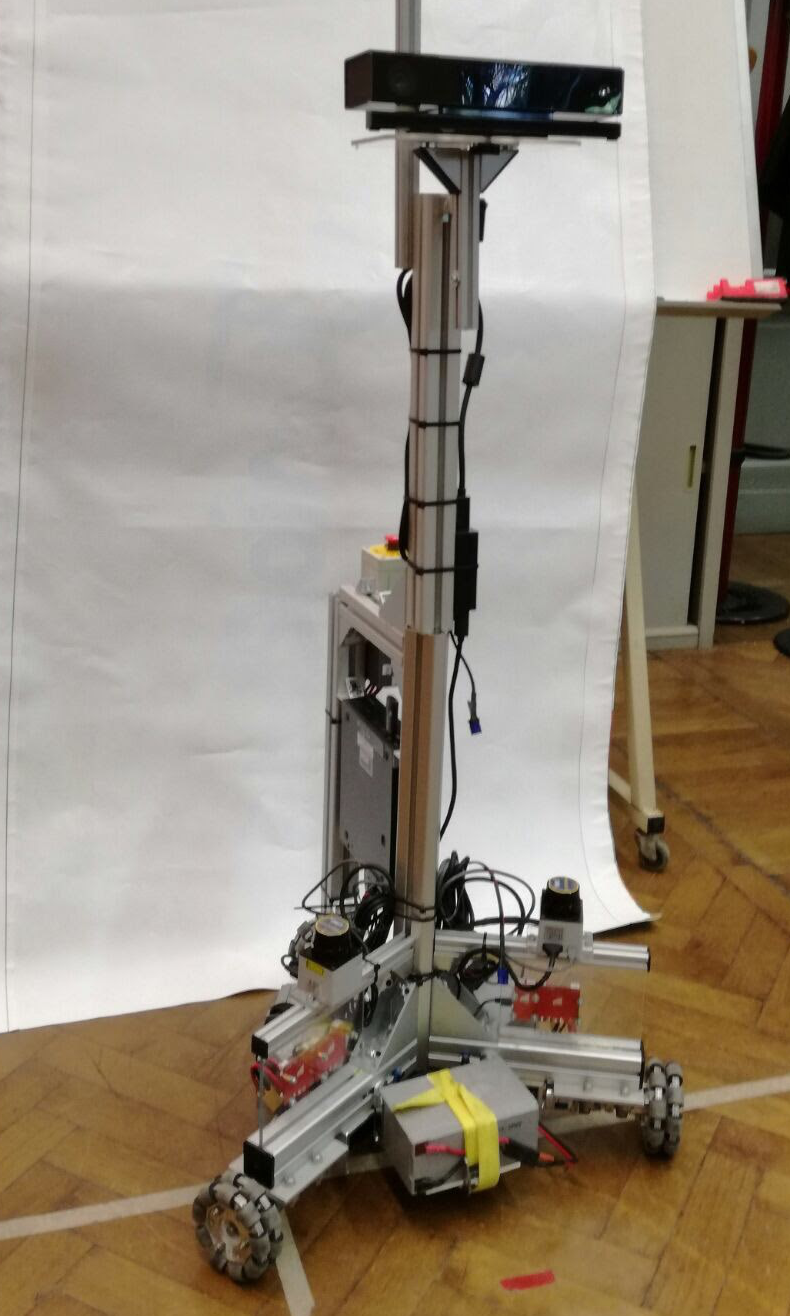
\includegraphics[draft=false, height=4cm,width=2.5cm]{images/03-foundation/structure}}}
        \caption{}
        \label{fig:aluminum_structure}
    \end{subfigure}
    ~
    \begin{subfigure}[b]{0.22\textwidth}
      	\centering
        \framebox{\parbox{2.5cm}{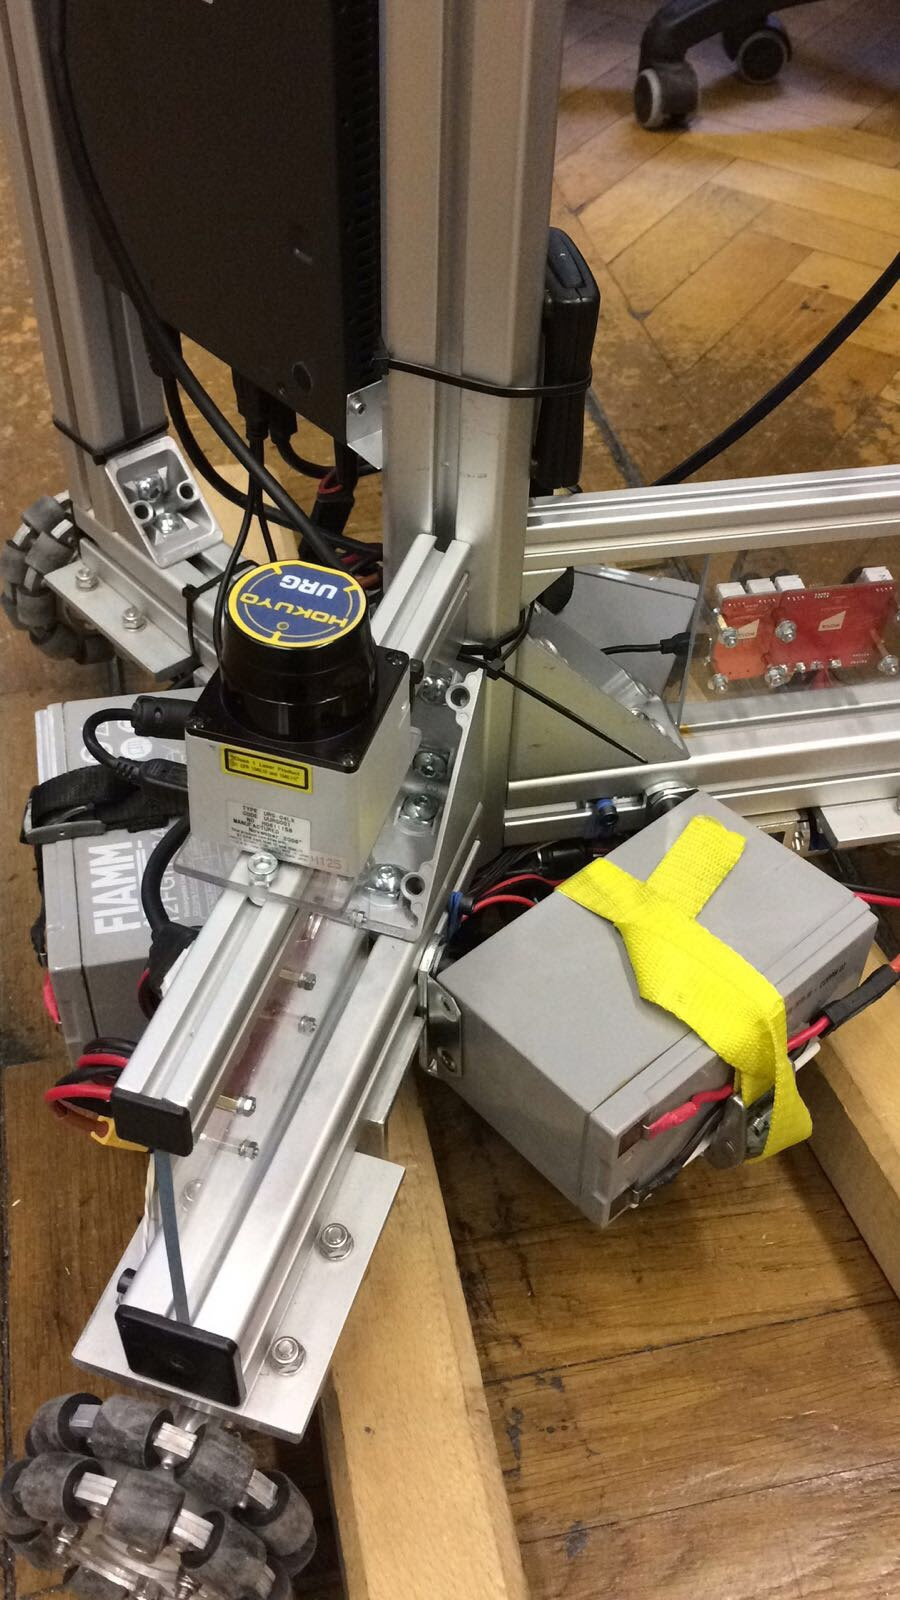
\includegraphics[draft=false,height=4cm,width=2.5cm]{images/03-foundation/structureII}}}
        \caption{}
        \label{fig:batteries}
    \end{subfigure}
    ~
    \begin{subfigure}[b]{0.22\textwidth}
      	\centering
        \framebox{\parbox{2.5cm}{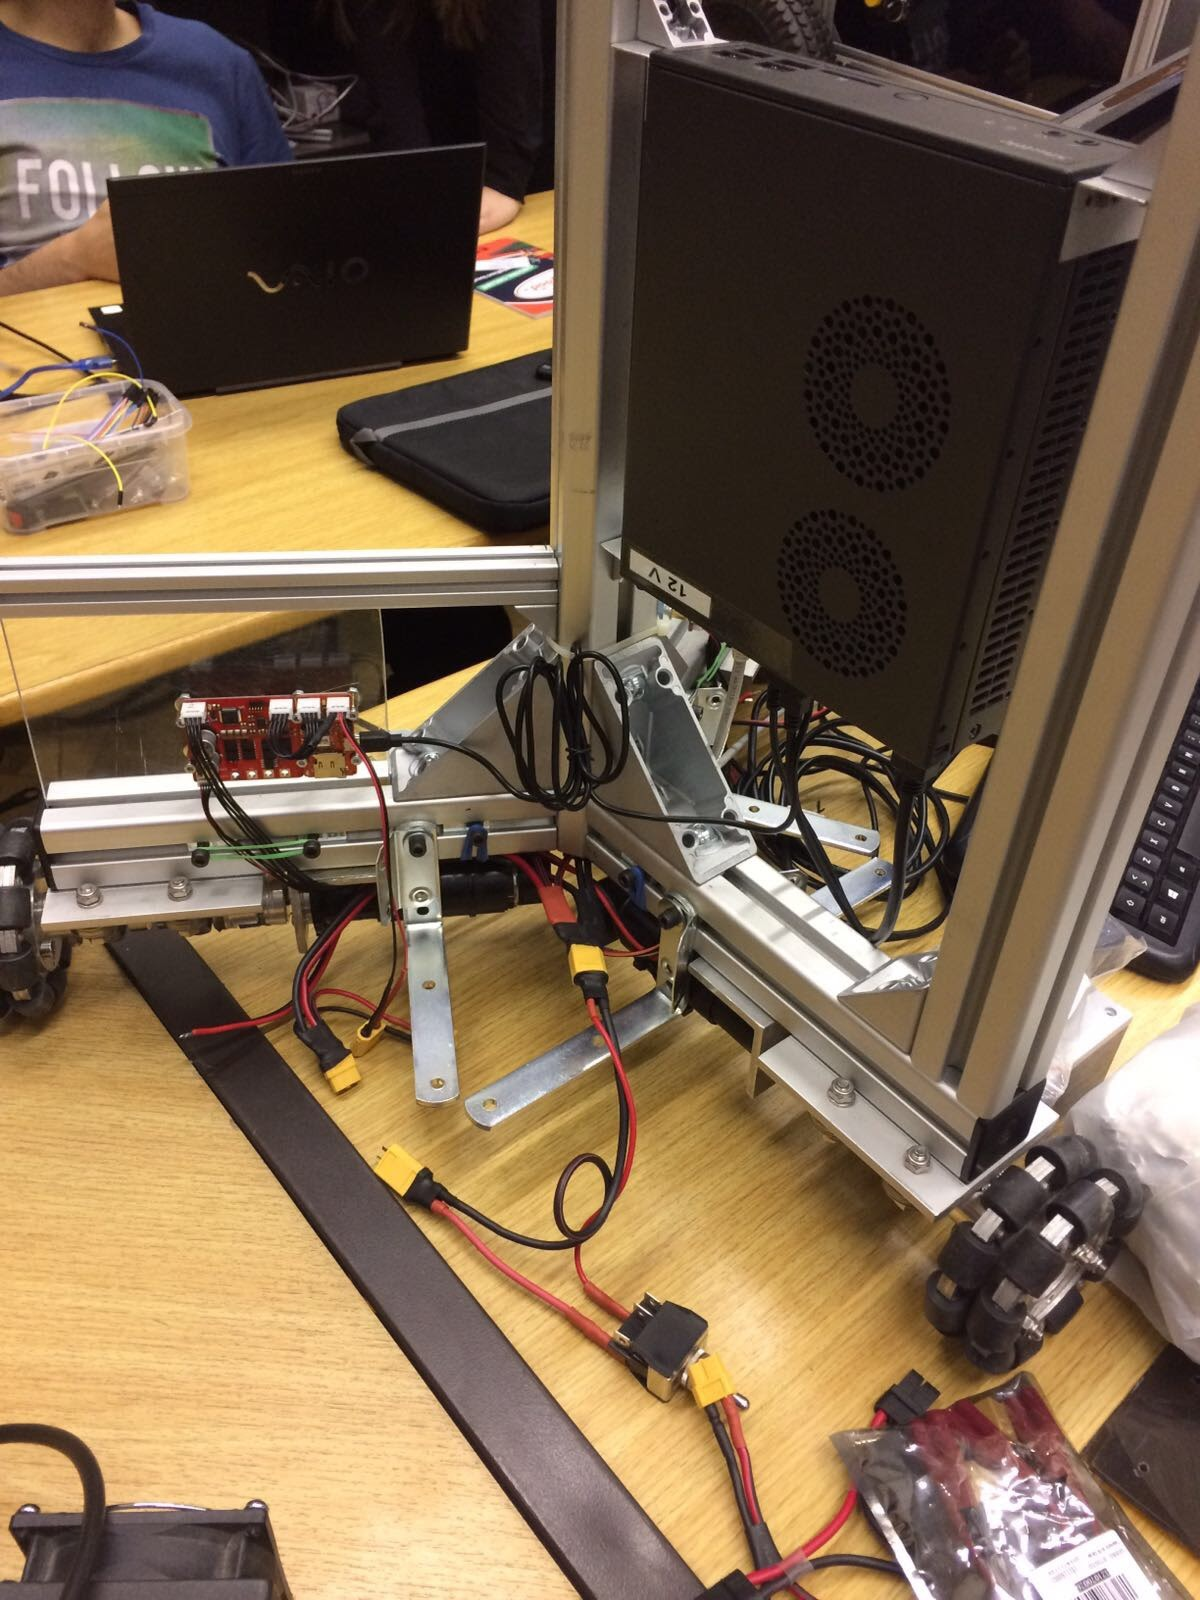
\includegraphics[draft=false,height=4cm,width=2.5cm]{images/03-foundation/structureIII}}}
        \caption{}
        \label{fig:computer}
    \end{subfigure}
    \caption{Structural details of our robot. The chassis is made of modular aluminum profiles from which rapid and easy prototyping is possible while retaining a good level of robustness. a) The full scale view of the robot (3rd version). b) a close-up view of one of the 2-D lasers and batteries (gray boxes). c) a close-up view of the vertical placement of computer (black box) and control board (red board).}
    \label{fig:structure_details}
\end{figure}

\subsection{Kinematics}

\subsection{Power distribution}

\section{Computing}

\subsection{Onboard computer}\label{onboard pc}
For computing a Shuttle XPC Slim DH270 was used. The device has a $190 \times 165 \times 43$~mm steel case, and weights $1.3$~kg.  The armature presents two holes for Kensington Locks and numerous threaded holes (M3) at both sides allowing for an easy placement. The operating system used was~\textit{Ubuntu 16.04.3 LTS (64bit)}. The computer had an Intel Core i7 and a RAM DDR4 memory of 16 GB .

\section{Control boards}
\label{novacore}
The low-level motors actuation and their interface between the ROS system have been realized with the Nova Core modules based on STM32-chip~\cite{noauthor_nova_nodate}, which implement ready to use components to fulfill robot prototyping requirements with plug \& play approach.  
The provided modules allow to control different type of motors that can be modeled as a second order system, where the input is the voltage applied to the motor armature and output variable is the motor angular speed. Futher details about the deployed boards are presented in figure~\ref{fig:boards}.


\begin{figure}[H]
  \centering
  \begin{subfigure}[b]{0.3\textwidth}
  \centering
      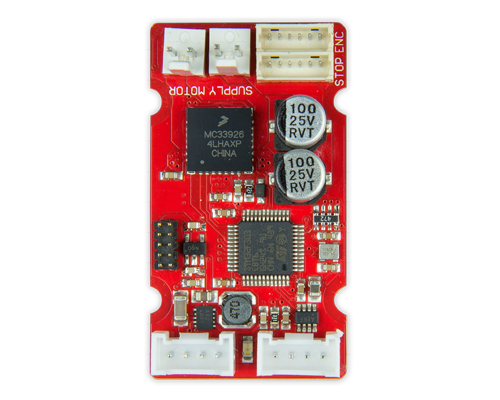
\includegraphics[width=3cm,height=3cm]{images/03-foundation/udc}
	\caption{}
  \end{subfigure}
  \begin{subfigure}[b]{0.3\textwidth}
  \centering
      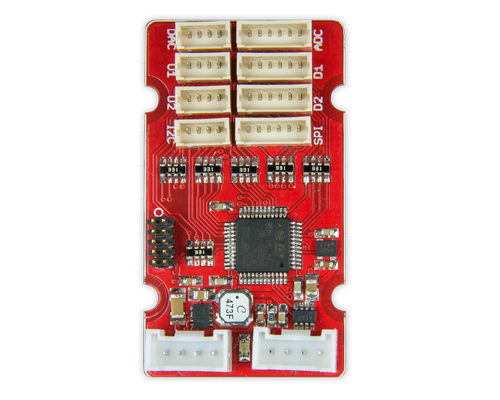
\includegraphics[width=3cm,height=3cm]{images/03-foundation/io}
	\caption{}
  \end{subfigure}
  \begin{subfigure}[b]{0.3\textwidth}
  \centering
      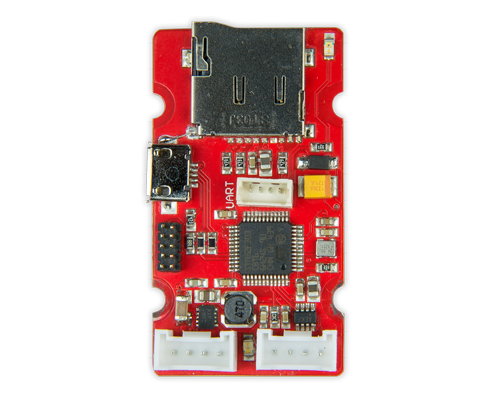
\includegraphics[width=3cm,height=3cm]{images/03-foundation/usb}
	\caption{}
	\label{fig:usb_board}
  \end{subfigure}
  \caption{a) UDC board (1 per each motor) capable of driving motors up to 70 W, with torque, speed, and position closed loop control. General attributes: 5-28V supply; 3A max (5A peak); current sense; encoder input; limit switch input; 25 x 45 mm in size. b) IO board (1 per each motor): Integrate existing hardware into the real-time Nova Core bus with analog and digital signals. General attributes: 8 digital GPIO;  4 analog inputs; 2 analog outputs; 2 UART; 1 I2C; 1 SPI; 25 x 45 mm in size. c) USB board (used for data collection) Interface the real-time Nova Core bus with a computer and logs data to microSD memory. General attributes: USB connector;  UART connector; microSD card slot; rosserial support; 25 x 45 mm in size.}
  \label{fig:boards}
\end{figure}
%ANDY all the technical details and names of devices could go in an appendix, while I'll leave here a functional description of robot and sensors, giving the characteristics that are functionally relevant, e.g., speed, omnidirectionality, range of sensors, their data rate, ...

\section{Navigation}
\subsection{\glsdesc{slam}}
\subsection{\glsdesc{oa}}

\section{Player perception and Tracking}
For opening the device, we have used libfreenect2\footnote{~\url{https://github.com/OpenKinect/libfreenect2} accessed on \today.}, a library for managing the Kinect\textsuperscript{\textregistered} device on Linux. We have then created a custom tracking node capable of estimating the player's position in two phases: First, color blob detection. Second, segmentation on the depth frame using \textit{region growing} algorithm for the purpose of detecting the player's body. Two features can be detected from this procedure: distance (relative to the robot) and contraction index. The first is calculated from the mean value of the depth pixels around the center of the blob. The latter is computed based on the subtraction of the occupied area with respect to the dimension of the bounding box that encompasses the segmented silhouette (see Figure~\ref{fig:segmenta}). This feature had been considered as a cue about the fact that the player was opening arms, so, possibly, actively participate to the game.

\begin{figure}[h]
  \centering 
  \begin{subfigure}[b]{0.3\textwidth}
		\centering
		\framebox{\parbox{3cm}{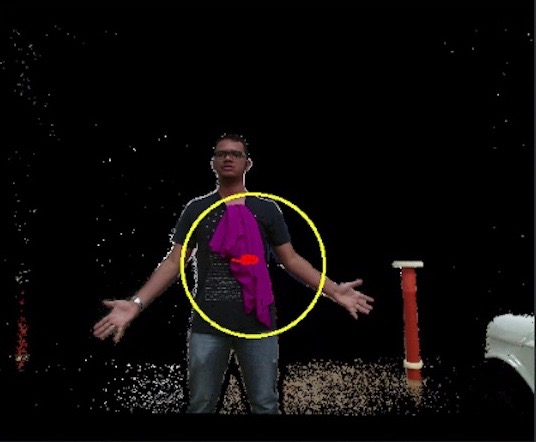
\includegraphics[draft=false,width=3cm, height=3cm]{images/03-foundation/point_cloud}}}
		\caption{}
  \end{subfigure}
  ~
  \begin{subfigure}[b]{0.3\textwidth}
		\centering
		\framebox{\parbox{3cm}{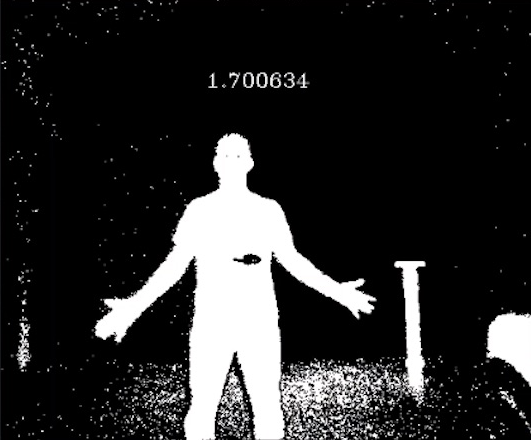
\includegraphics[draft=false,width=3cm, height=3cm]{images/03-foundation/depth}}}
		\caption{}
  \end{subfigure}
  ~
  \begin{subfigure}[b]{0.3\textwidth}
		\centering
		\framebox{\parbox{3cm}{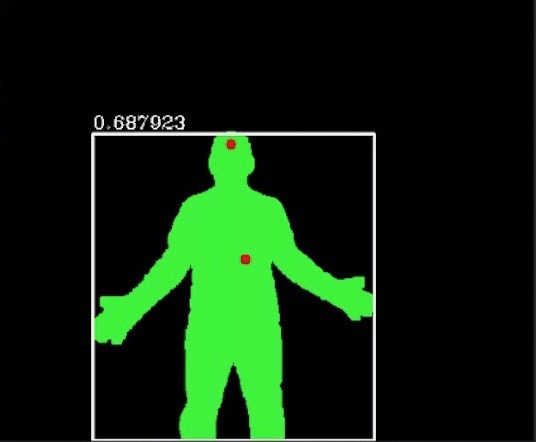
\includegraphics[draft=false,width=3cm, height=3cm]{images/03-foundation/segmentation}}}
		\caption{}
  \end{subfigure}
  \caption{Example of frames processed by our algorithm. a) Point cloud showing the center of the detected (light-purple) color blob. b) Depth frame. The number showed above the user correspond to his estimated distance relative to the robot (in meters). c) Segmentation results. The number above is the contraction index defined in the interval [0,1] and can be used as a measure of body contraction.}\label{fig:segmenta}
   \label{segmentacao}
\end{figure}